\section{Introdução}
\begin{figure}[H]
    \centering
    \caption{Imagem teste}
    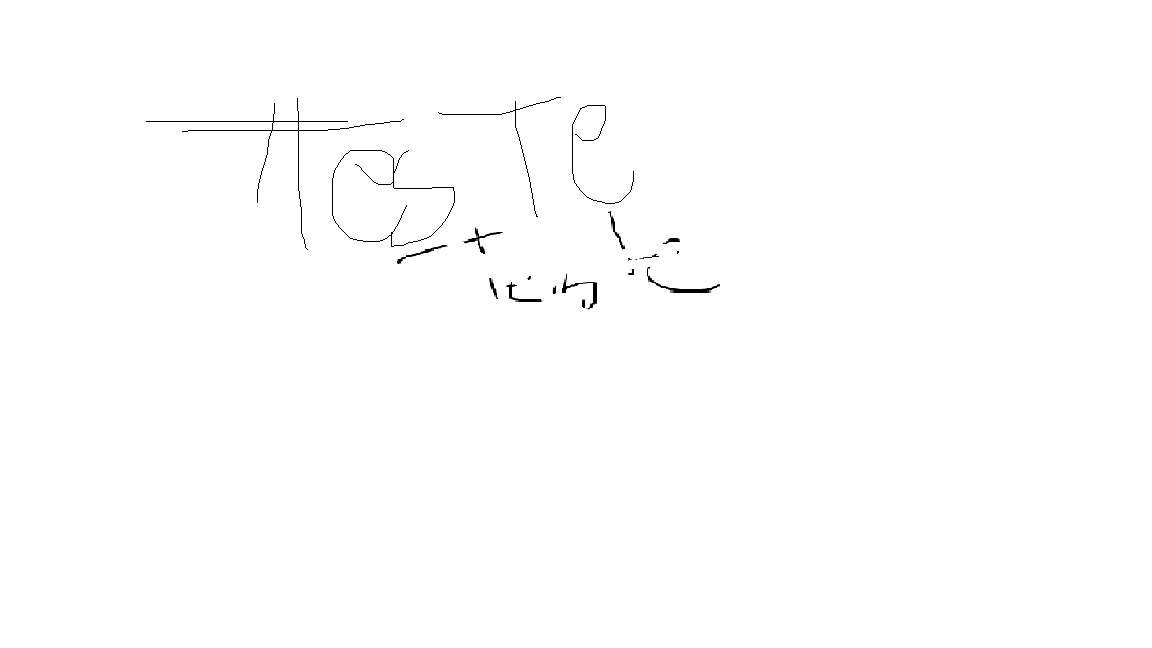
\includegraphics[width=0.5\linewidth]{images/Teste.png}\\
    \fonteimagem{Fonte: autor}
    \label{fig:figura-teste}
\end{figure}

\begin{table}[H]
    \centering
    \caption{Tabela teste}
    \begin{tabular}{|c|c|c|}
        \hline
        Column 1 & Column 2 & Column 3 \\
        \hline
        Data 1 & Data 2 & Data 3 \\
        \hline
        Data 4 & Data 5 & Data 6 \\
        \hline
    \end{tabular}\\
    \fonteimagem{Fonte: autor}
    \label{tabular:teste1}
\end{table}

\begin{lstlisting}[caption={Código teste},language=Java,label=codigo-teste]
public class HelloWorld {
    public static void main(String[] args) {
        // Print "Hello, World!" to the console
        System.out.println("Hello, World!");
    }
}
\end{lstlisting}

\newpage

Podemos referenciar figura \ref{fig:figura-teste}, tabela \ref{tabular:teste1}, código \ref{codigo-teste} \cite{doe2021example}.

Segundo \textcite{smith2020example}. Aqui temos um exemplo de referencia no rodapé \footcite{smith2020example}.

Um exemplo de citação direta, segundo \textcite[p.~30]{miller2019example} diz-se: ``Lorem ipsum dolor sit amet, consectetur adipiscing elit. Nunc rutrum mi eget nulla fermentum, in vestibulum diam dignissim. In hac habitasse platea dictumst. Donec in arcu dui. Fusce at nisl ac tortor tempor interdum. Proin interdum dignissim mi, vitae bibendum turpis vestibulum dictum. Fusce diam augue, lobortis vel tincidunt vitae, auctor quis orci. Integer condimentum luctus dui luctus placerat. Mauris facilisis ligula leo, eget mollis magna facilisis sit ame''.